\documentclass[11pt,a4paper]{article}

\usepackage[T1]{fontenc}
\usepackage[utf8]{inputenc}
\usepackage{lmodern}
\usepackage[english]{babel}
\usepackage{geometry}
\geometry{margin=2.4cm}
\usepackage{graphicx}
\usepackage{microtype}
\usepackage{xcolor}
\usepackage{listings}
\usepackage{hyperref}
\hypersetup{
  colorlinks=true, linkcolor=blue!60!black, urlcolor=blue!60!black,
  citecolor=blue!60!black, pdftitle={baboon-acoustics user documentation},
  pdfauthor={anonymized for review}}
\usepackage{enumitem}
\setlist{itemsep=2pt, topsep=4pt}

\lstset{
  language=Python,
  basicstyle=\ttfamily\small,
  keywordstyle=\color{blue!70!black},
  commentstyle=\color{green!45!black},
  stringstyle=\color{orange!70!black},
  showstringspaces=false,
  frame=single,
  framerule=0.3pt,
  rulecolor=\color{black!30},
  backgroundcolor=\color{black!3},
  breaklines=true,
  columns=fullflexible,
  captionpos=b,
}

\newcommand{\pkg}{\texttt{baboon\_acoustics}}

\title{\vspace{-1.2cm}\textbf{baboon-acoustics}\\[2mm]
\large Formant, F0, glottal-source and vocal-tract-length\\
analysis of baboon vocalizations\\[4mm]
\normalsize User documentation (v1.0)}
\author{anonymized for review}
\date{September 2026}

\begin{document}
\maketitle

\begin{abstract}
\noindent This document is the user guide of the \pkg{} Python package,
the supplementary code of the article \emph{Re-analysis of formant
trajectories in a chacma baboon wahoo vocalization} (anonymized for
review). It introduces the underlying acoustic concepts in plain
language, walks through the installation, follows a complete tutorial on
the provided recordings, documents every public function of the package,
and answers frequently asked questions. No prior signal-processing
knowledge is assumed.
\end{abstract}

\tableofcontents

\section{Introduction}

\subsection{What this package does}

When a mammal vocalizes, the lungs drive air through the larynx, where
the vocal folds chop the flow into pulses (the \emph{glottal source}),
and the resulting sound is filtered by the cavities of the throat, mouth
and nose (the \emph{vocal tract}). This is the classic
\emph{source--filter theory} of vocal production. The package analyses
recordings along these two layers:

\begin{itemize}
\item \textbf{Formants} are the resonant frequencies of the vocal tract.
They appear as peaks in the spectral envelope and are conventionally
numbered F1, F2, F3, \ldots{} from the lowest upwards. Their spacing
depends on the length and shape of the tract, so they carry information
about the caller's anatomy (and, when articulation occurs, about
vowel-like gestures).
\item \textbf{The fundamental frequency (F0)} is the repetition rate of
the glottal pulses; it is the acoustic correlate of pitch.
\item \textbf{The vocal tract length (VTL)} can be estimated from the
formant pattern: for a tube closed at one end, the resonances fall near
$F_i = (2i-1)\,c / (4\,\mathrm{VTL})$ with $i = 1, 2, 3, \ldots$ and $c$
the speed of sound (Reby \& McComb 2003).
\item \textbf{The glottal source waveform} itself can be recovered by
\emph{inverse filtering}: removing the vocal-tract resonances from the
recorded signal leaves (an estimate of) the glottal flow. Its shape
reveals the phonation type and, in the case studied in the article,
nonlinear phenomena such as subharmonics and deterministic chaos.
\end{itemize}

\subsection{Two ways of measuring formants}

\paragraph{Praat's Burg method (module \texttt{formants\_praat}).}
Linear predictive coding (LPC) fits an all-pole filter to a short
analysis window; the poles are reported as formant candidates. The
implementation is Praat's \emph{Burg} algorithm, accessed through the
Parselmouth interface (Jadoul et al.\ 2018). The main parameter is the
number of poles $N$: too few, and neighbouring formants merge; too many,
and extra poles lock onto harmonics of the source rather than true
resonances. For a tract of about 17\,cm analysed up to 5.5\,kHz,
classical theory predicts roughly 5--6 poles; the article shows on the
baboon wahoo that $N=4$ (the setting of the original study) only tracks
the central part of the call, while $N=6$ is needed for its initial and
final parts (Figure~\ref{fig:figure1}).

\paragraph{IAIF inverse filtering (module \texttt{formants\_iaif}).}
Plain LPC assumes a spectrally flat source, which the glottal source is
not. \emph{Iterative adaptive inverse filtering} (IAIF; Alku 1991)
alternates between estimating the glottal contribution (low-order LPC)
and the vocal tract (high-order LPC), each iteration refining the other.
The result is both a cleaner vocal-tract envelope --- whose peaks are
the formants --- and the glottal waveform itself. IAIF needs longer
windows (about 90\,ms) and more computation, but it exposes source
dynamics that LPC hides; on the wahoo it reveals strong departures from
a regular periodic source.

\begin{figure}[t]
\centering
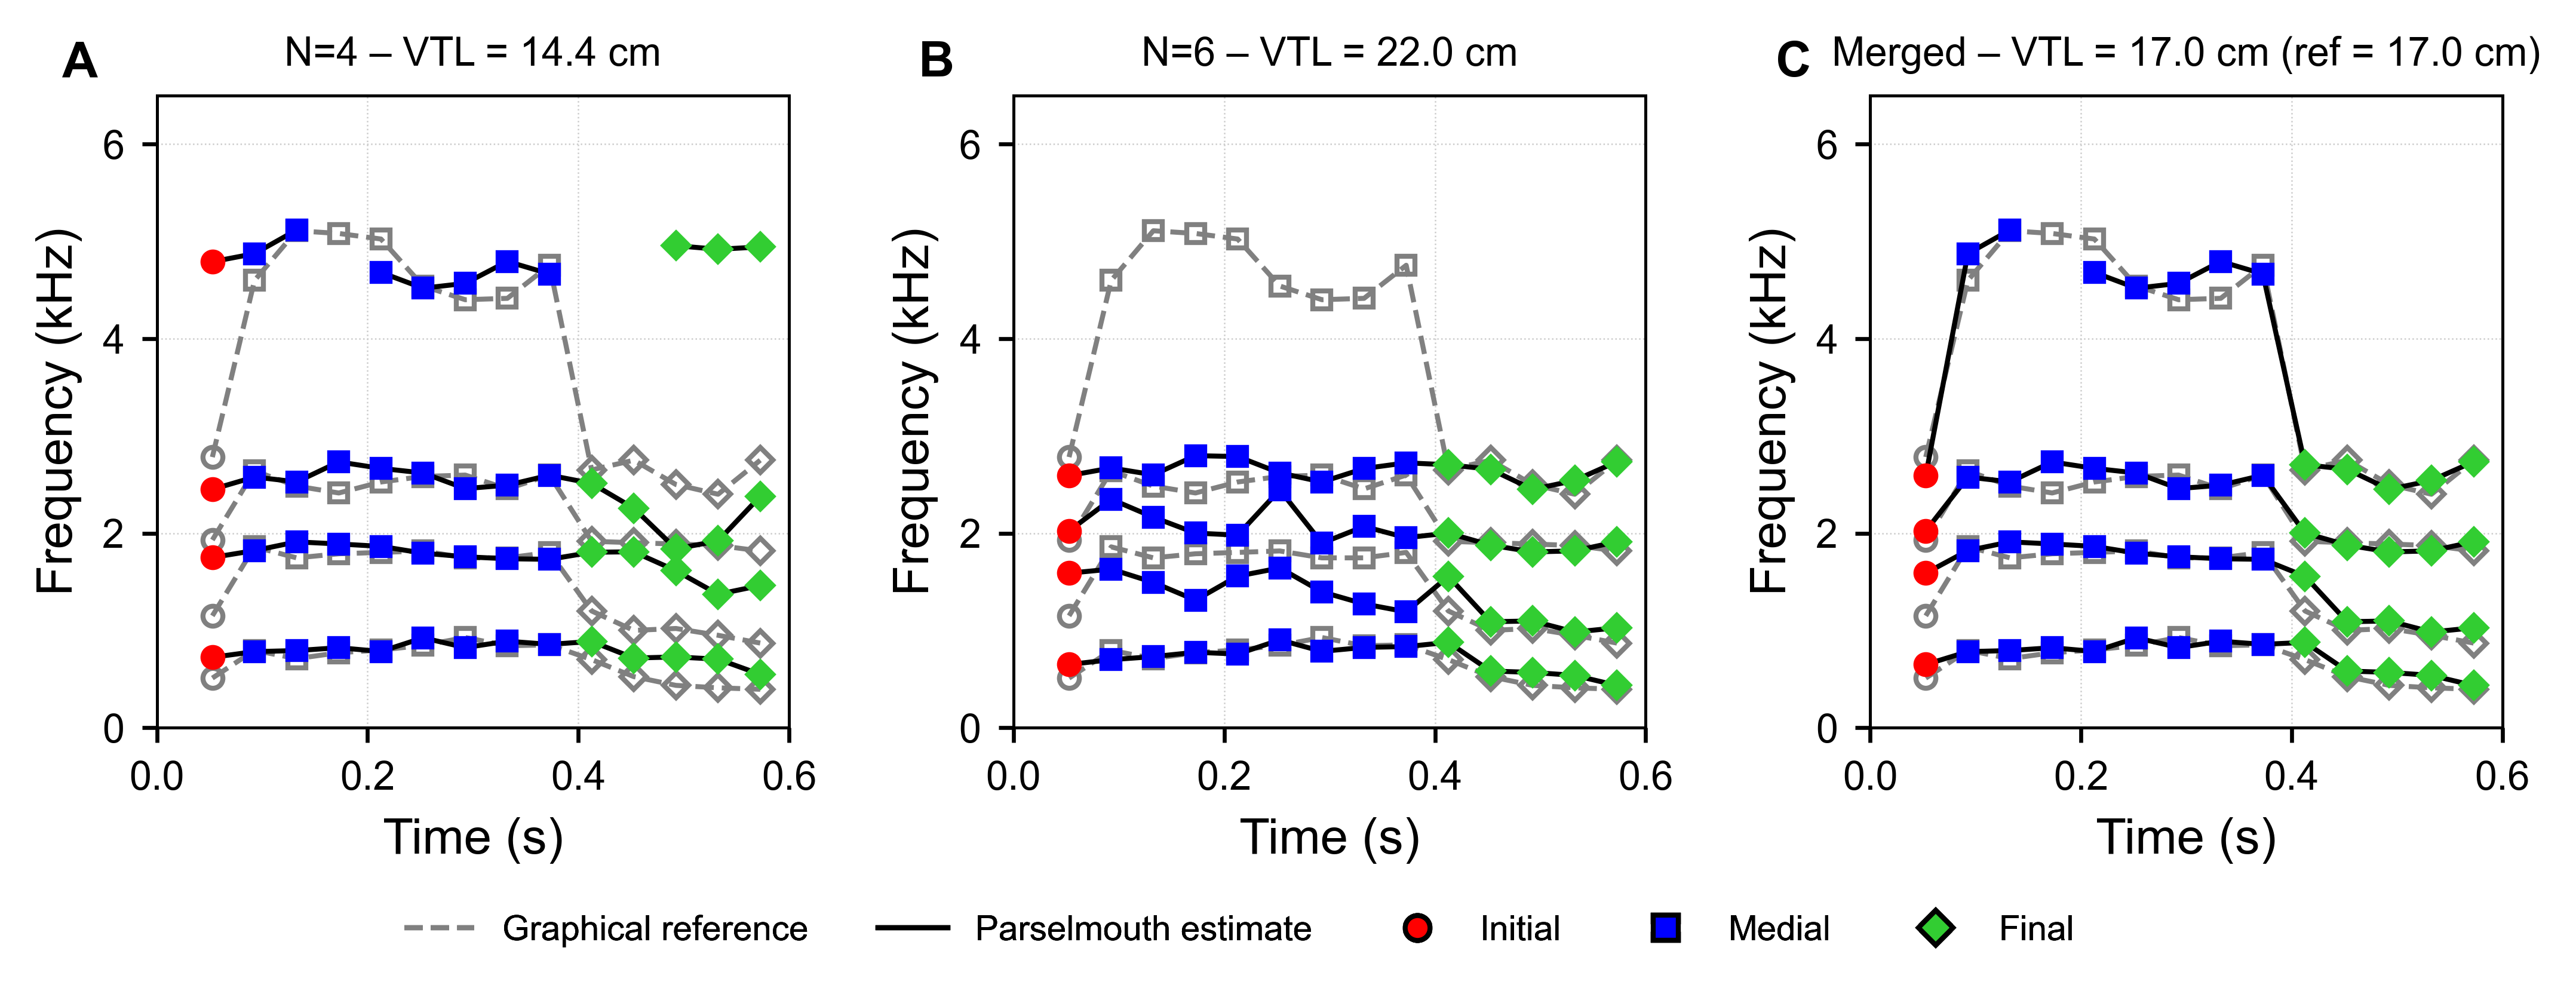
\includegraphics[width=\textwidth]{figures/Figure1.png}
\caption{Formant re-analysis of the wahoo (output of
\texttt{scripts/make\_figure1.py}). Panels (A) and (B): Parselmouth
tracks with $N=4$ and $N=6$ poles (grey dashed lines: reference data
digitized from Bo\"e et al.\ 2026). Panel (C): merged trajectory using
the optimal $N$ per segment. The $N{=}4$ setting only suits the central
segment; each panel title gives the corresponding VTL estimate.}
\label{fig:figure1}
\end{figure}

\section{Installation}

\pkg{} requires \textbf{Python 3.9 or newer} and four packages:

\begin{lstlisting}[language=bash]
git clone https://github.com/<your-account>/baboon-acoustics.git
cd baboon-acoustics
python -m pip install -r requirements.txt
\end{lstlisting}

\begin{itemize}
\item \texttt{numpy}, \texttt{scipy} --- numerical work and filtering;
\item \texttt{matplotlib} --- figures;
\item \texttt{praat-parselmouth} --- embeds the Praat sound engine; you
do \emph{not} need to install Praat separately.
\end{itemize}

Verify the installation with the test suite (about 30 seconds):

\begin{lstlisting}[language=bash]
python -m unittest discover -s tests
\end{lstlisting}

The package is used in place: scripts and examples add the repository
root to \texttt{sys.path} automatically, so simply run them from the
repository folder.

\section{Tutorial}

This tutorial reproduces the workflow of the article on the provided
recordings: \texttt{data/wahoo\_4.wav} (a 0.67\,s chacma baboon
\emph{wahoo} call, 44.1\,kHz) and \texttt{data/The\_Baboon\_Bark.wav}
(16\,s of barks, stereo). Everything shown here is assembled in
\texttt{examples/example\_analysis.py}, which can be run as-is.

\subsection{Step 1 --- load a recording}

\begin{lstlisting}
from baboon_acoustics import load_audio

samples, fs = load_audio("data/wahoo_4.wav")
\end{lstlisting}

\texttt{load\_audio} returns a mono, floating-point waveform and its
sampling frequency. Multi-channel files are reduced to the first
channel; recordings at other rates are resampled to 44.1\,kHz
(the default \texttt{target\_fs}); with \texttt{normalize=True} the
waveform is scaled to a peak amplitude of 1. Pass
\texttt{normalize=False} when absolute amplitudes matter (glottal-wave
displays).

\subsection{Step 2 --- track formants with Praat}

\begin{lstlisting}
from baboon_acoustics import extract_praat_formants

times, formants = extract_praat_formants("data/wahoo_4.wav",
                                         n_formants=4)
F1_hz = formants[0]        # first-formant track
F1_khz = F1_hz / 1000.0    # kHz, as plotted in the article
\end{lstlisting}

The result is an array of shape \texttt{(n\_formants, n\_frames)} in
Hz; \texttt{NaN} marks frames where Praat found no value. Frames are
40\,ms apart by default (\texttt{time\_step}); the analysis ceiling
(\texttt{formant\_ceiling}, default 5500\,Hz) and the pre-emphasis
frequency (50\,Hz) follow the settings of the article.

\subsection{Step 3 --- estimate the vocal tract length}

\begin{lstlisting}
from baboon_acoustics import reby_mccomb_vtl

vtl_cm = reby_mccomb_vtl(formants)
print(f"VTL = {vtl_cm:.1f} cm")
\end{lstlisting}

Every valid measurement of every formant contributes one point
(order, frequency), orders being the odd integers $1, 3, 5, 7, \ldots$
for F1, F2, F3, F4, \ldots{} A least-squares line through the origin
provides the slope, and $\mathrm{VTL} = c/(4b)$ with $c = 350$\,m/s.
On \texttt{wahoo\_4.wav} the merged trajectory of the article yields
about 17.0\,cm --- versus 14.4\,cm ($N{=}4$) and 22.0\,cm ($N{=}6$)
taken separately, a first indication that formant tracking, not
anatomy, drives the spread.

\subsection{Step 4 --- estimate F0}

\begin{lstlisting}
from baboon_acoustics import estimate_f0_praat

times, f0, strength = estimate_f0_praat("data/wahoo_4.wav")
\end{lstlisting}

This runs Praat's autocorrelation pitch analysis. With the default
\texttt{use\_prefilter=True}, the signal first passes through a
Gaussian low-pass filter that emulates the \emph{filtered
autocorrelation} of recent Praat versions; on calls with strong
subharmonics (the ``wa'' part of the wahoo), the plain autocorrelation
of older versions often locks onto F0/2. Comparing both modes is a
quick diagnostic for such nonlinearities:

\begin{lstlisting}
_, f0_raw, _ = estimate_f0_praat("data/wahoo_4.wav",
                                 use_prefilter=False)
\end{lstlisting}

A second, source-based estimator, \texttt{estimate\_f0\_from\_gn()},
measures F0 from the autocorrelation of a glottal waveform (step 6).

\subsection{Step 5 --- sliding IAIF analysis}

\begin{lstlisting}
from baboon_acoustics import iaif_sliding_analysis

result = iaif_sliding_analysis(samples, fs, n_formants=4)
result.times          # frame times (s)
result.formants       # (n_formants, n_frames) in Hz
result.f0_track       # F0 per frame (Hz, NaN if unvoiced)
result.glottal_db     # spectrogram of the IAIF glottal source (dB)
result.envelope_db    # IAIF vocal-tract envelope |Hvt| (dB)
\end{lstlisting}

The signal is sliced into 4096-sample Hann windows (93\,ms, 75\,%
overlap) and each window is decomposed by IAIF.
Figure~\ref{fig:multipanel} shows the complete six-panel output this
analysis feeds: spectrograms with $N{=}4$ and $N{=}6$ Praat overlays
(A, B), the F1--F2 trajectory against the Maximal Acoustic Space (MAS)
of the species (C, D), the IAIF source with its F0 track (E), and the
vocal-tract envelope with the IAIF formants (F).

\begin{figure}[t]
\centering
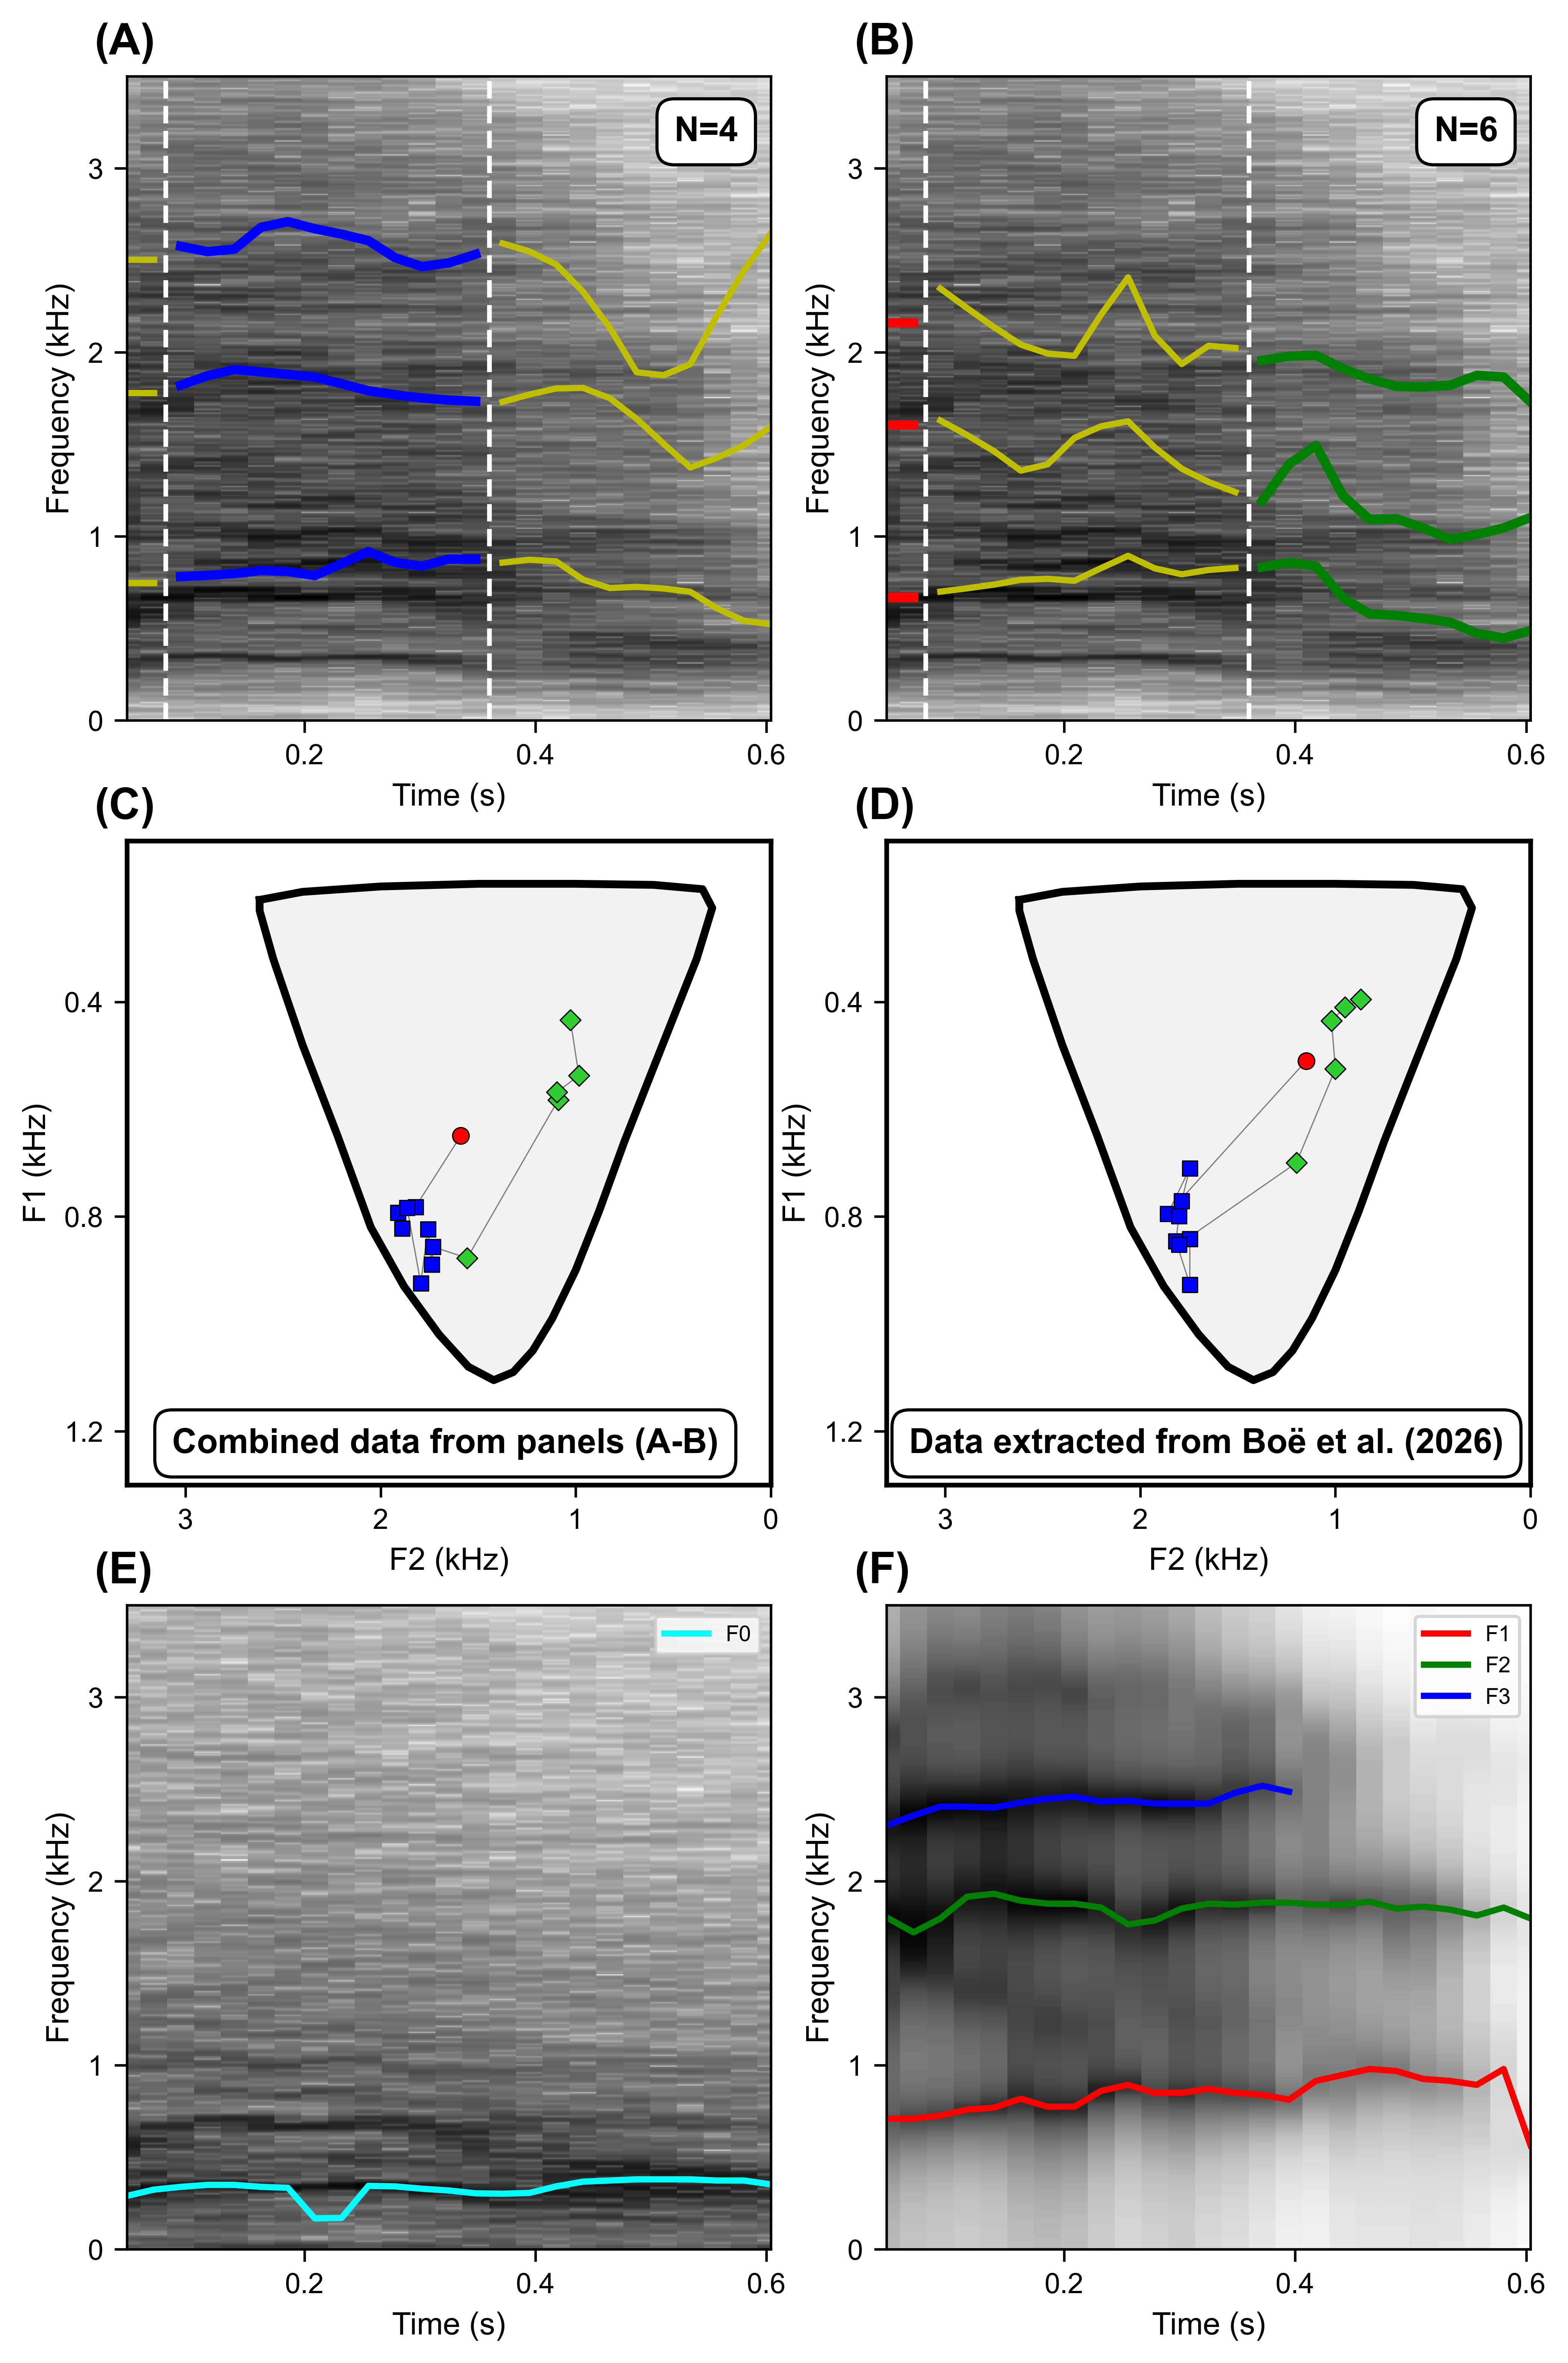
\includegraphics[width=0.72\textwidth]{figures/analysis_3x2_panels.png}
\caption{Six-panel analysis of \texttt{wahoo\_4.wav} (output of
\texttt{scripts/make\_figure\_multipanel.py}). The F1--F2 trajectories
of panels (C)--(D) are drawn over the Maximal Acoustic Space contour of
the chacma baboon; markers encode the position within the call (circle:
initial frame; squares: medial; diamonds: final).}
\label{fig:multipanel}
\end{figure}

\subsection{Step 6 --- glottal source analysis}

\begin{lstlisting}
from baboon_acoustics import (load_audio,
                              extract_glottal_pulse,
                              extract_glottal_train)

x, fs = load_audio("data/wahoo_4.wav", normalize=False)

t_pulse, pulse = extract_glottal_pulse(x, fs, 0.26, 0.34)
t_train, train = extract_glottal_train(x, fs)
\end{lstlisting}

\texttt{extract\_glottal\_pulse} isolates a single glottal cycle from a
stable segment (here 260--340\,ms, the vowel-like middle of the call);
\texttt{extract\_glottal\_train} reconstructs the full pulse train by
overlap-add of windowed IAIF estimates
(Figure~\ref{fig:glottal}, top). Phase portraits of the train
(\texttt{plot\_phase\_portrait}) expose amplitude and period
irregularities: closed loops indicate periodic phonation, spread or
folded trajectories indicate subharmonics or chaos
(Figure~\ref{fig:glottal}, bottom left).

\begin{figure}[t]
\centering
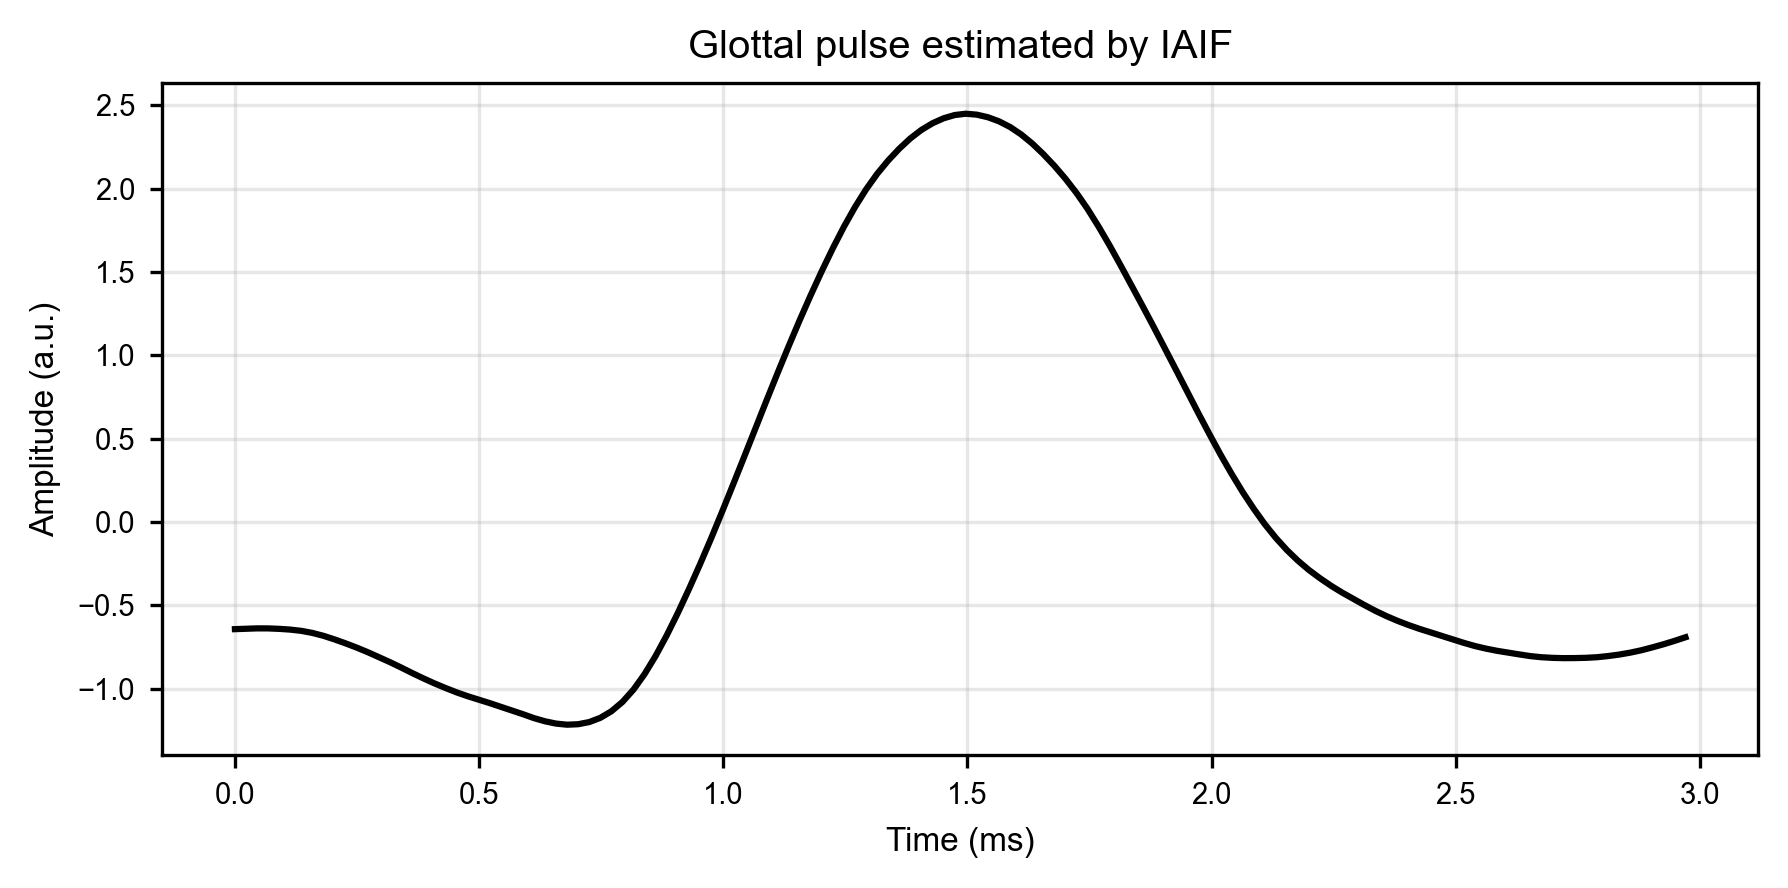
\includegraphics[width=0.485\textwidth]{figures/glottal_pulse.png}
\hfill
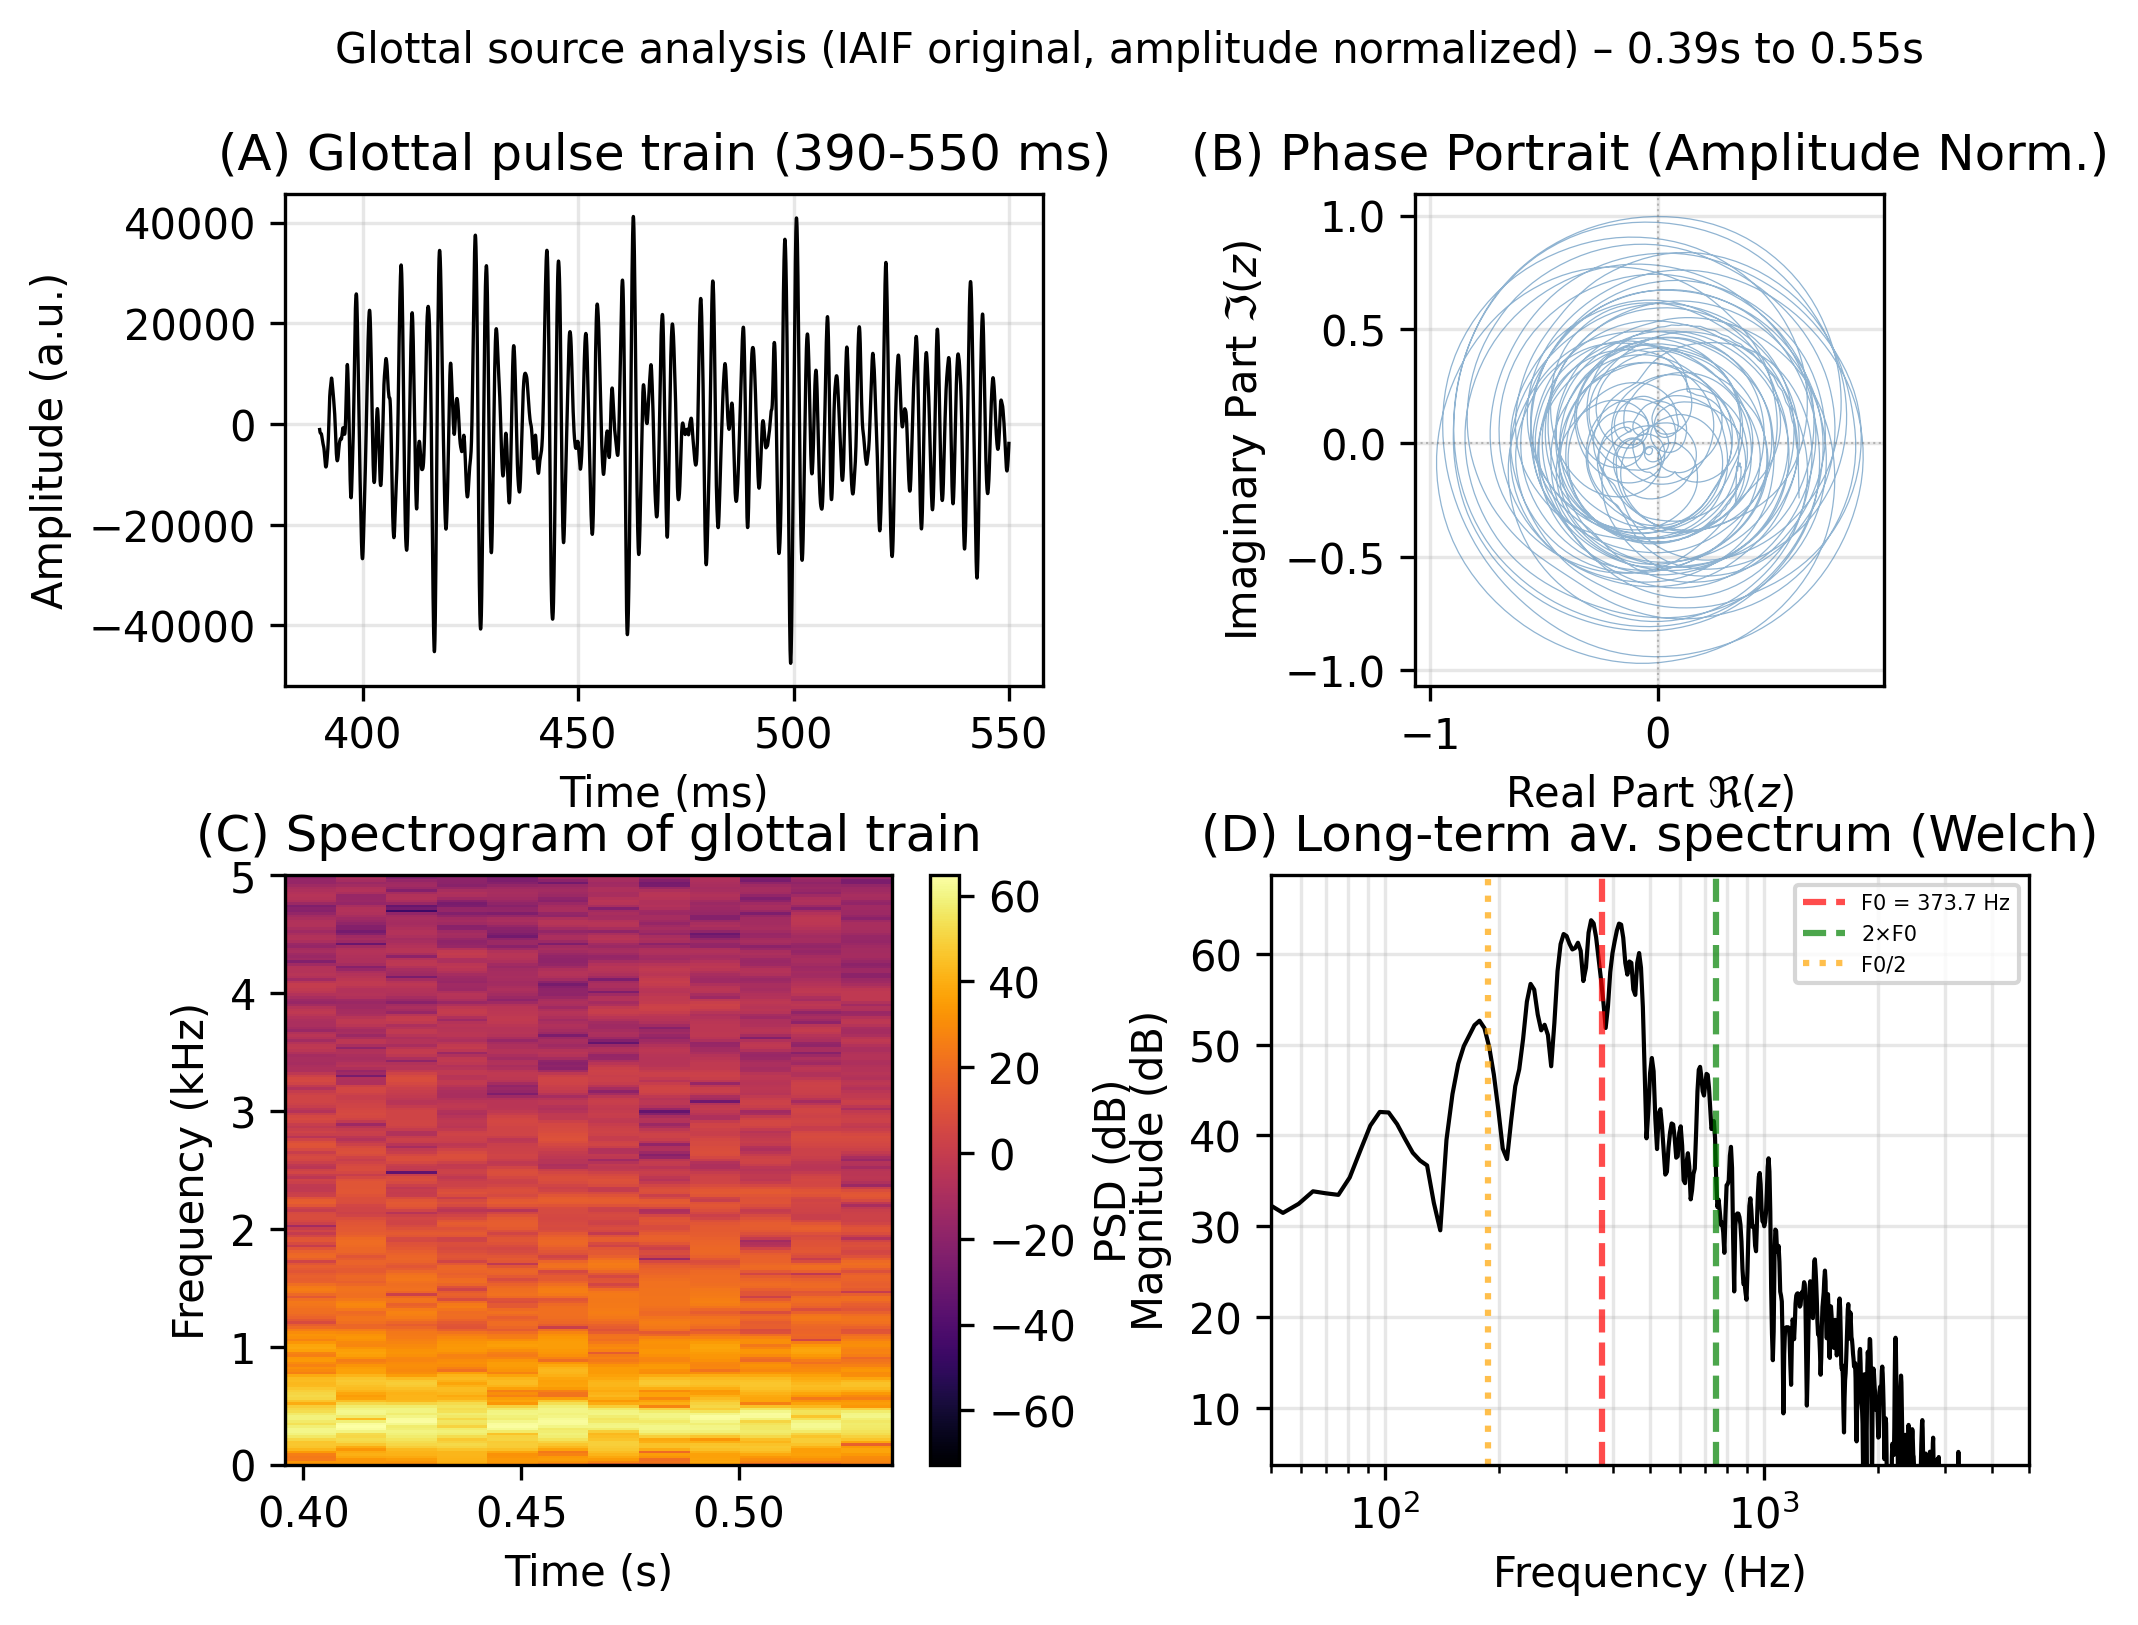
\includegraphics[width=0.485\textwidth]{figures/glottal_train_analysis_hoo.png}
\caption{Left: single glottal pulse estimated by IAIF. Right:
four-panel glottal-source analysis of the ``hoo'' segment (output of
\texttt{scripts/make\_figure\_glottal.py}): waveform, Hilbert phase
portrait, spectrogram, and long-term average spectrum with F0 markers.}
\label{fig:glottal}
\end{figure}

\subsection{Step 7 --- F0 contour and the article's exclusion criteria}

Finally, \texttt{scripts/make\_figure\_f0.py} writes the F0 contour of
the filtered autocorrelation to a CSV table and a plot
(Figure~\ref{fig:f0}). On the wahoo, the contour exceeds 300\,Hz
throughout, and F1 falls below $1.5 \times$ F0 over most of the ``hoo''
segment --- the two exclusion criteria discussed in the article.

\begin{figure}[t]
\centering
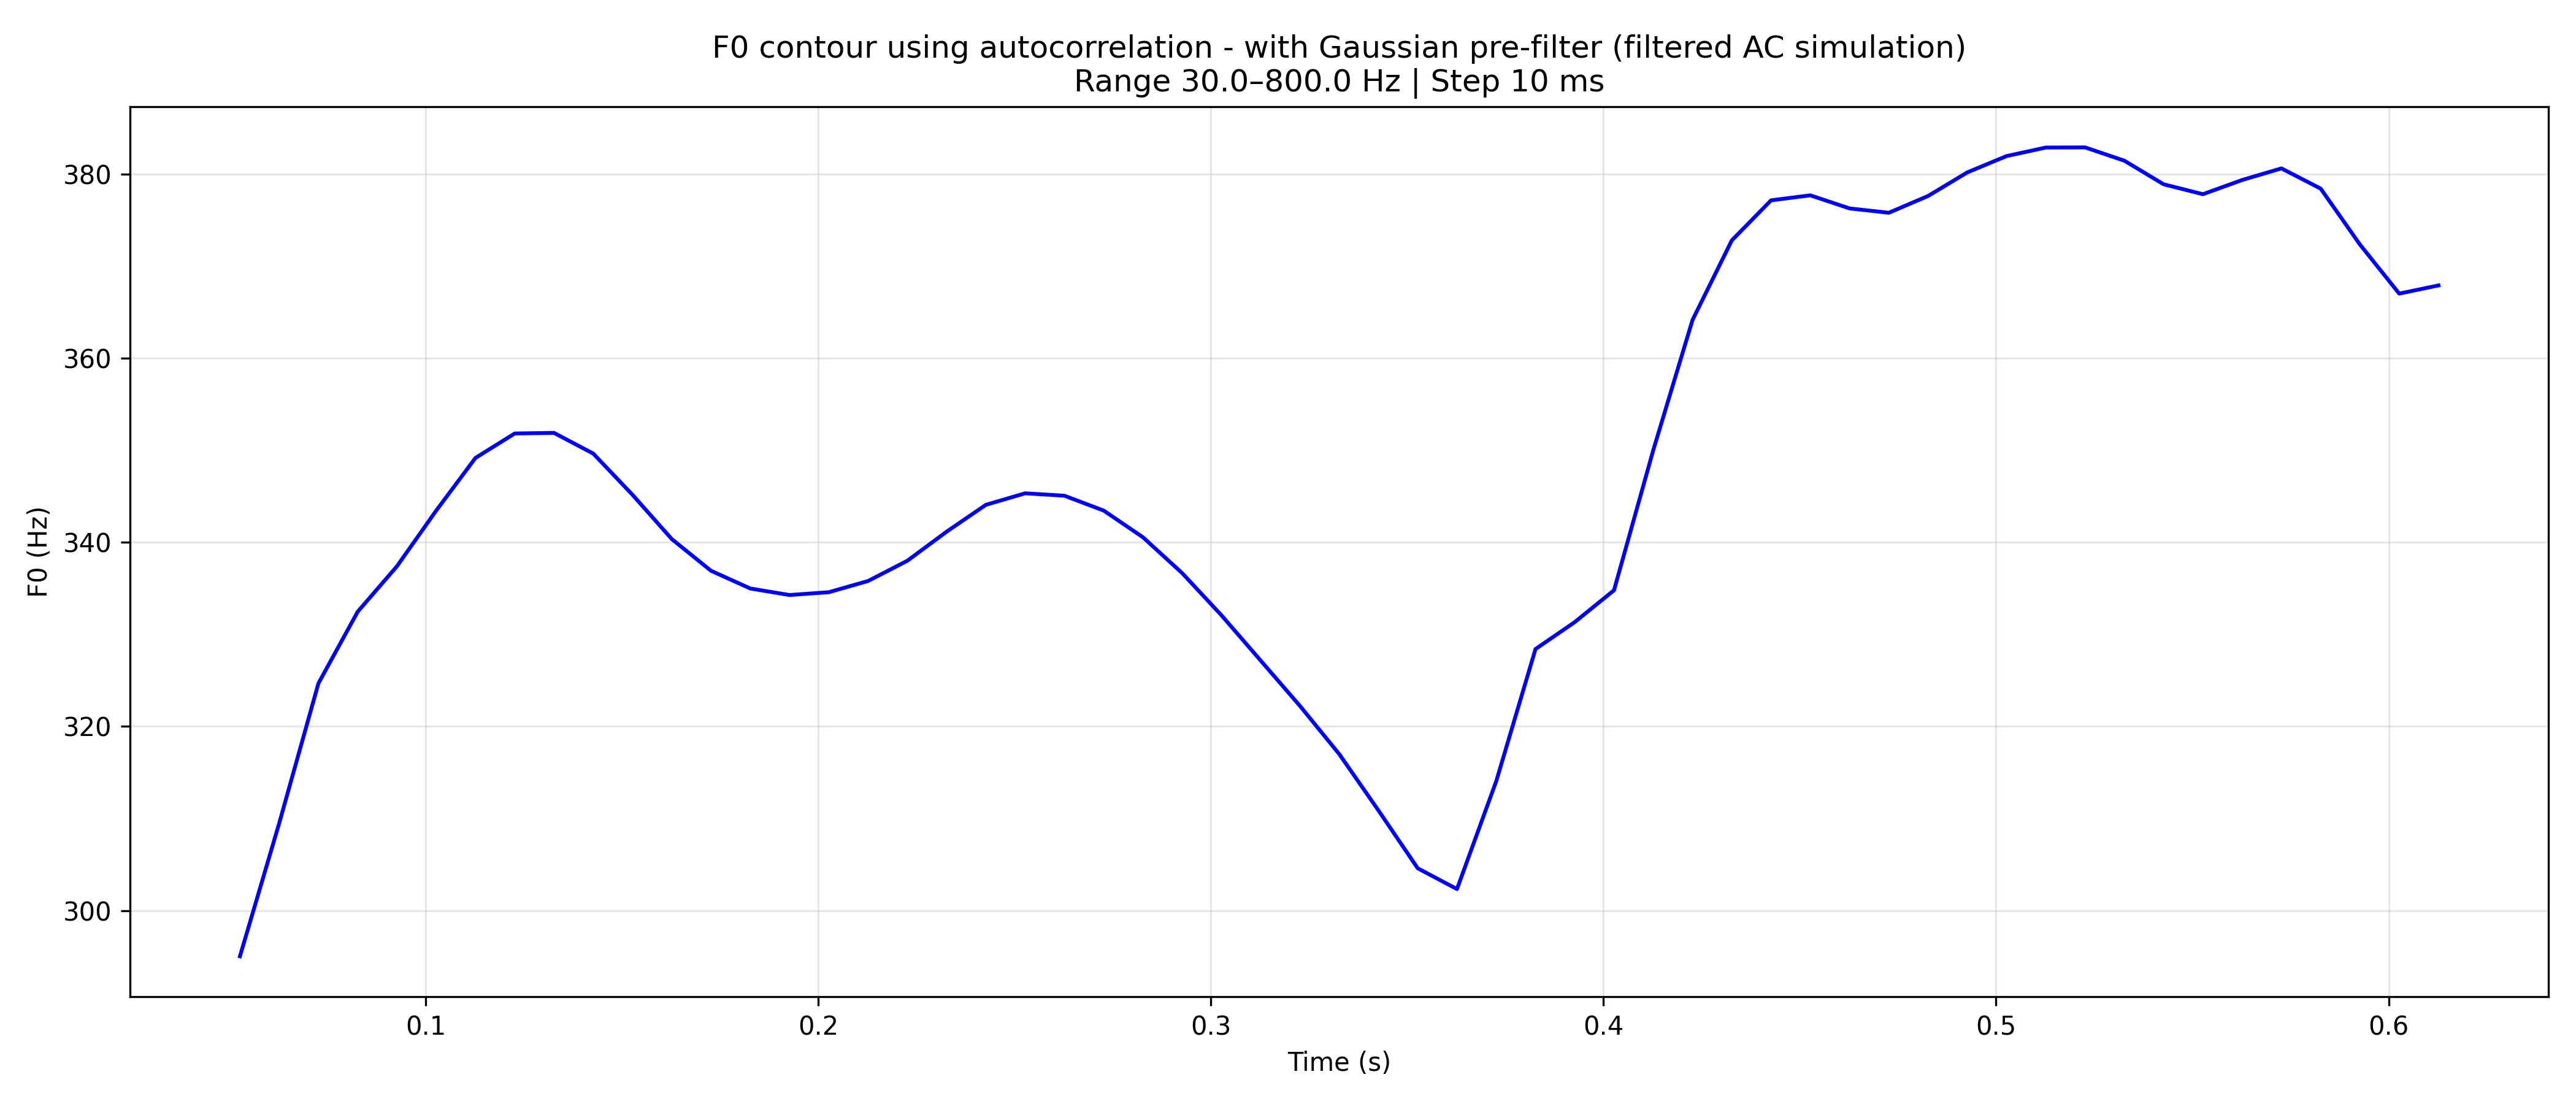
\includegraphics[width=0.9\textwidth]{figures/wahoo_4_f0_filtered_ac.png}
\caption{F0 contour of \texttt{wahoo\_4.wav} obtained with the Gaussian
pre-filtered autocorrelation (output of \texttt{scripts/make\_figure\_f0.py}).}
\label{fig:f0}
\end{figure}

\section{API reference}

All frequencies are in Hz, times in seconds, amplitudes arbitrary
unless stated. Every function is documented in its docstring;
\texttt{help(module)} or \texttt{help(function)} shows the same text
inside Python.

\subsection{\texttt{baboon\_acoustics.audio\_io} --- loading audio}

\begin{description}[style=nextline, leftmargin=1.2em]
\item[\texttt{load\_audio(path, target\_fs=44100, normalize=True)}]
Reads a WAV file, keeps the first channel of multi-channel recordings,
converts to float64, optionally peak-normalizes to $[-1, 1]$, and
resamples to \texttt{target\_fs} with a polyphase filter when needed.
Returns \texttt{(samples, fs)}.
\end{description}

\subsection{\texttt{baboon\_acoustics.formants\_praat} --- Praat/Burg formants}

\begin{description}[style=nextline, leftmargin=1.2em]
\item[\texttt{extract\_praat\_formants(audio\_path, n\_formants,
fs\_target=44100, formant\_ceiling=5500, window=0.040,
time\_step=0.040, pre\_emphasis=50)}]
Runs Praat's ``To Formant (burg)''. Returns \texttt{(times, formants)}
with \texttt{formants} of shape \texttt{(n\_formants, n\_frames)} in Hz
(\texttt{NaN} where undefined).
\item[\texttt{interpolate\_formants(source\_times, formants,
target\_times)}]
Linearly resamples tracks onto a new time grid, ignoring NaN frames and
extending NaN outside the valid range.
\item[\texttt{fill\_leading\_nan(track)}]
Replaces a leading NaN (Praat's half-filled first window) by the first
valid value.
\end{description}

\subsection{\texttt{baboon\_acoustics.formants\_iaif} --- IAIF}

\begin{description}[style=nextline, leftmargin=1.2em]
\item[\texttt{lpc\_levinson(x, order)}]
LPC coefficients of a frame via FFT autocorrelation and the
Levinson--Durbin recursion. Returns \texttt{(coefficients, energy)}.
\item[\texttt{lpc\_spectrum\_db(lpc\_coeffs, error\_variance,
n\_fft=4096, fs=44100)}]
Magnitude response of the LPC all-pole filter, in dB.
\item[\texttt{iaif\_frame(frame, fs, vt\_order=60)}]
One IAIF decomposition: returns the vocal-tract LPC filter, its
prediction error, and the glottal-flow derivative estimate.
\item[\texttt{get\_frame\_formants(frame, fs, vt\_order=60,
n\_formants=4, fmax=3500, min\_prominence=2.5,
min\_dist\_hz=150)}]
Formants of one frame as the \texttt{n\_formants} lowest of the
\texttt{n\_formants~+~2} most prominent peaks of the IAIF envelope
below \texttt{fmax}; pads with NaN.
\item[\texttt{iaif\_sliding\_analysis(x, fs, n\_formants=4, ...)}]
Sliding-window IAIF over the whole signal; returns an
\texttt{IaifResult} named tuple (\texttt{times}, \texttt{freqs},
\texttt{spectrogram\_db}, \texttt{glottal\_db}, \texttt{envelope\_db},
\texttt{f0\_track}, \texttt{formants}).
\end{description}

\subsection{\texttt{baboon\_acoustics.f0} --- fundamental frequency}

\begin{description}[style=nextline, leftmargin=1.2em]
\item[\texttt{estimate\_f0\_from\_gn(glottal, fs, f0\_min=50,
f0\_max=500, ac\_threshold=0.3)}]
F0 from the autocorrelation of a glottal waveform; returns NaN for
unvoiced frames.
\item[\texttt{gaussian\_lowpass\_filter(samples, fs, cutoff=800,
attenuation=0.03)}]
Frequency-domain Gaussian pre-filter used to emulate Praat's filtered
autocorrelation.
\item[\texttt{estimate\_f0\_praat(audio\_path, use\_prefilter=True,
time\_step=0.01, pitch\_floor=30, pitch\_ceiling=800, ...)}]
Praat autocorrelation pitch analysis; returns
\texttt{(times, f0, strength)} for the voiced frames only.
\end{description}

\subsection{\texttt{baboon\_acoustics.vtl} --- vocal tract length}

\begin{description}[style=nextline, leftmargin=1.2em]
\item[\texttt{reby\_mccomb\_vtl(formants, c=350.0)}]
Single VTL estimate (cm) from formant tracks in Hz --- a
\texttt{(n\_formants, n\_frames)} array or a sequence of tracks; NaNs
ignored, any number of formants accepted. Returns NaN below two valid
values.
\end{description}

\subsection{\texttt{baboon\_acoustics.glottal} --- glottal source}

\begin{description}[style=nextline, leftmargin=1.2em]
\item[\texttt{extract\_glottal\_pulse(x, fs, t\_start, t\_end,
vt\_order=60, f0\_min=50, f0\_max=500)}]
One glottal cycle from a quasi-stationary segment (Hamming window,
autocorrelation period, cut around the largest excursion). Returns
\texttt{(t, pulse)} or \texttt{(None, None)} if the segment is shorter
than 1024 samples.
\item[\texttt{extract\_glottal\_train(x, fs, vt\_order=60,
win\_len=4096, hop=1024)}]
Full glottal train by overlap-add of windowed IAIF estimates, trimmed
at the edges.
\item[\texttt{normalize\_amplitude(signal, fs, cutoff=50, order=4,
eps=1e-6)}]
Removes floating DC and flattens the slow envelope (Butterworth
low-pass of the signal and of its magnitude); trims 512 samples at each
end to discard filter transients.
\end{description}

\subsection{\texttt{baboon\_acoustics.plotting} --- figures}

\begin{description}[style=nextline, leftmargin=1.2em]
\item[\texttt{set\_journal\_style(base\_size=8, tick\_size=7,
legend\_size=6, linewidth=0.8, titlesize=None, embed\_fonts=False)}]
Compact Arial style of the article figures.
\item[\texttt{add\_panel\_label(ax, label, ...)}]
Bold panel letter, e.g.\ ``(A)''.
\item[\texttt{setup\_frequency\_axis(ax)}]
Time--frequency axes (s vs.\ kHz, 0--3.5\,kHz) shared by the
spectrogram panels.
\item[\texttt{plot\_f1f2\_trajectory(ax, f1\_khz, f2\_khz, markers,
colors, mas\_f1\_khz, mas\_f2\_khz)}]
F1--F2 trajectory over the Maximal Acoustic Space contour (F2 axis
reversed, vowel-chart convention).
\item[\texttt{plot\_phase\_portrait(ax, signal, fs, ...)}]
Hilbert analytic-signal portrait (optionally amplitude-normalized).
\item[\texttt{plot\_formant\_comparison\_panel(ax, times, formants,
reference, title, letter, vtl\_value, vtl\_reference=None)}]
One panel of Figure~1: estimated tracks and markers over a grey dashed
reference.
\end{description}

\section{Reproducing the article figures}

From the repository root:

\begin{lstlisting}[language=bash]
python scripts/make_figure1.py               # Figure1.png
python scripts/make_figure_multipanel.py     # 6-panel figure + glottal pulse
python scripts/make_figure_glottal.py        # glottal train, "hoo" segment
python scripts/make_figure_glottal.py --segment wa   # ... "wa" segment
python scripts/make_figure_f0.py             # F0 table (CSV) + plot
\end{lstlisting}

Outputs land in \texttt{figures/}. On the provided data the numerical
outputs are exact (the F0 table matches the archived reference to a
relative difference below $10^{-9}$) and the figures are visually
identical to those of the article.

\section{FAQ and common pitfalls}

\paragraph{How many formants ($N$) should I request?}
A rule of thumb from quarter-wave theory: $N \approx 2 \cdot
\mathrm{VTL} \cdot \mathrm{F_{max}} / c + 1$. For a baboon tract of
17\,cm and $F_{max} = 5.5$\,kHz this gives $N \approx 5.5$, i.e.\ try
$N=5$ or 6. Extract with two or three neighbouring values and compare
(\texttt{extract\_praat\_formants} is fast): if a formant track jumps by
hundreds of Hz between settings, it is unstable --- as happens with
$N=4$ on the wahoo. If your tracks look like a comb of evenly spaced
peaks, $N$ is too high and the extra poles follow harmonics.

\paragraph{Formants below 1.5$\times$F0 are unreliable.}
Praat (and LPC in general) cannot separate a formant from a strong
nearby harmonic. Track F0 as well (\texttt{estimate\_f0\_praat}) and
discard frames where $F_1 < 1.5\,F_0$ --- one of the exclusion criteria
applied in the article.

\paragraph{Which sampling rate?}
Recordings are resampled to 44.1\,kHz by default because the IAIF
parameters (window of 4096 samples, vocal-tract order 60) are expressed
at that rate. For recordings of signals far below 20\,kHz you may pass
\texttt{target\_fs=16000} to \texttt{load\_audio} --- the Praat branch
then needs matching \texttt{formant\_ceiling} (e.g.\ 5000 for baboons,
well below the Nyquist of any audio recording).

\paragraph{The file is long --- IAIF is slow.}
The sliding analysis costs roughly 0.3\,s per 0.1\,s of audio at 44.1
kHz on a typical laptop. Slice the waveform first
(\texttt{x = x[int(1.2 * fs):int(2.0 * fs)]}) and analyse the segment
of interest; Praat-based functions, by contrast, handle minutes of
audio in seconds (the 16\,s bark file takes a few seconds).

\paragraph{F0 looks locked at half (or twice) the expected value.}
This is the classic subharmonic (or octave) error of autocorrelation
pitch trackers on calls with nonlinear dynamics. Compare
\texttt{estimate\_f0\_praat(..., use\_prefilter=True)} and
\texttt{use\_prefilter=False}; systematic discrepancies indicate
subharmonics in the source --- inspect the glottal train
(\texttt{extract\_glottal\_train}) and its phase portrait.

\paragraph{I get NaN formants / NaN VTL.}
NaNs are normal where the analysis cannot find a value (low signal
energy, unvoiced frames). \texttt{reby\_mccomb\_vtl} ignores them, and
returns NaN only when fewer than two valid measurements remain in the
whole input --- check your segment bounds if that happens.

\paragraph{Can I analyse species other than baboons?}
Yes. Only the MAS contour and the segment boundaries in the figure
scripts are baboon-specific; every analysis function is generic. Adjust
\texttt{fmax} / \texttt{formant\_ceiling} and the F0 search range to
your species.

\section{References}

\begin{itemize}
\item Alku, P. (1991). Glottal wave analysis with pitch synchronous
iterative adaptive inverse filtering. \emph{Proceedings of Eurospeech
1991}, 1081--1084.
\item Bo\"e, L.-J., Laporte, M., Sawallis, T.\,R., Badin, P., \&
Schwartz, J.-L. (2026). Stalking the wild formant: How to reliably
measure formants in primate vocalizations. \emph{International Journal
of Primatology}. \url{https://doi.org/10.1007/s10764-026-00551-4}
\item Jadoul, Y., Thompson, B., \& de Boer, B. (2018). Introducing
Parselmouth: A Python interface to Praat. \emph{Journal of Phonetics},
71, 1--15.
\item Reby, D., \& McComb, K. (2003). Anatomical constraints generate
honesty: acoustic cues to age and weight in the roars of red deer.
\emph{Animal Behaviour}, 65(3), 519--530.
\end{itemize}

\end{document}
